\section{Horizon Length}

In order to determine what horizon length is needed to optimize the path, several paths were optimized with horizon lengths varying from $10$ to $140$, spaced by $10$. One piecewise linear and one curved $45\degree$ turn was optimized using the different horizon lengths. The results of these optimizations can be seen in Figures \ref{fig:horizon_uav_position} and \ref{fig:horizon_camera_position}.

The results for the two paths are very similar; the longer horizon length, the better tracking of the path. The MPC starts turning earlier than the ground track to compensate for the sideways shift in the camera position caused by the roll, and the aircraft straightens out from the turn later for the same reason.

For the shorter horizon lengths the MPC runs into problems because it hasn't planned far enough ahead when the turn begins. Since it does not look far into the future the aircraft is still straight above the path when the turn begins. At that point it is too late to start altering the aircrafts position to ensure that the camera stays on the path, so the MPC uses a roll angle in the opposite direction to keep observing the path. This in turn leads to the aircraft turning left, worsening the situation and making the problem more and more difficult. In some cases this causes the roll angle to become very high, causing the MPC to lose control and the aircraft loses height.

Upon closer inspections it can be seen that when the horizon length reaches $90$, there are no more big unwanted motions in the system. As the horizon length reaches $110$ the optimized paths are almost identical, but increasing the horizon length still increases the accuracy of the path tracking. The optimization is time consuming, and as seen in Figure \ref{fig:horizon_duration} the time it takes to optimize the paths increases exponentially. For this reason a horizon length of $110$ will be used for the rest of the simulations, as this gives an accurate path tracking for a relatively short computation time.

%% Position figures

\begin{figure}
	\makebox[\textwidth][c]{
	\subfloat[Subfigure 1][Linear $45\degree$ turn.]{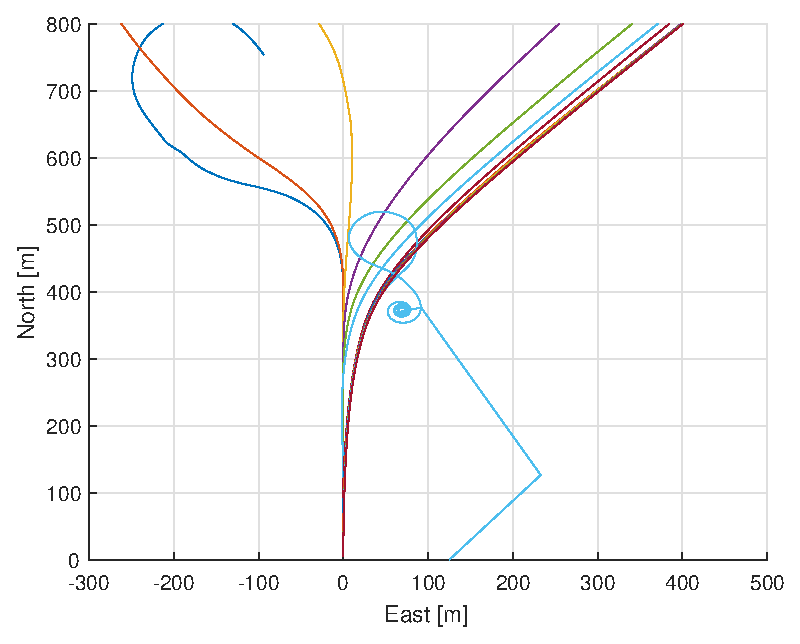
\includegraphics[width=0.8\textwidth, keepaspectratio=true]{../../results/opt/horizon/lin_45deg/fig/uav_position.eps}}}
	\qquad
	\makebox[\textwidth][c]{
	\subfloat[Subfigure 2][Curved $45\degree$ turn with $200$m radius.]{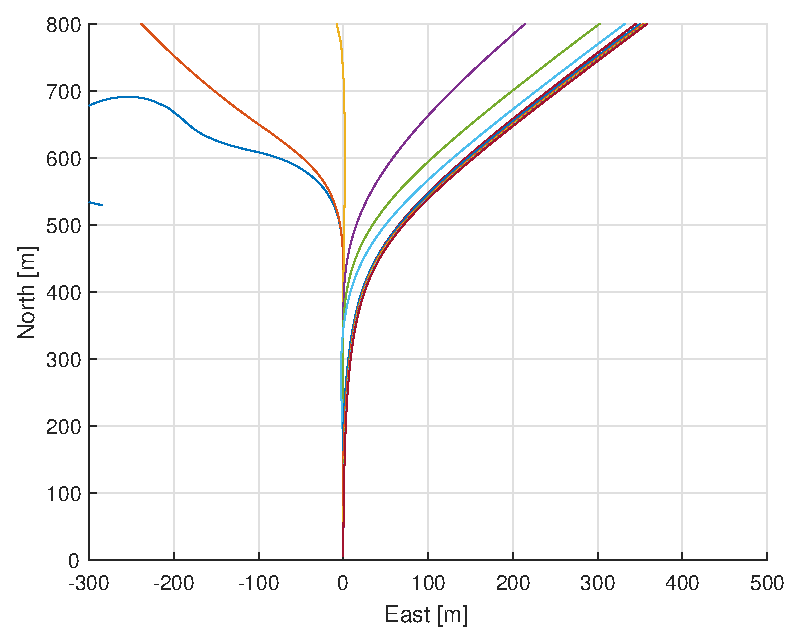
\includegraphics[width=0.8\textwidth, keepaspectratio=true]{../../results/opt/horizon/cur_45deg_200m/fig/uav_position.eps}}}
	\caption{The position of the UAV during the two turns with horizon lengths varying from 10 to 140.}
	\label{fig:horizon_uav_position}
\end{figure}


%% Camera position
\begin{figure}
	\makebox[\textwidth][c]{
	\subfloat[Subfigure 1][Linear $45\degree$ turn.]{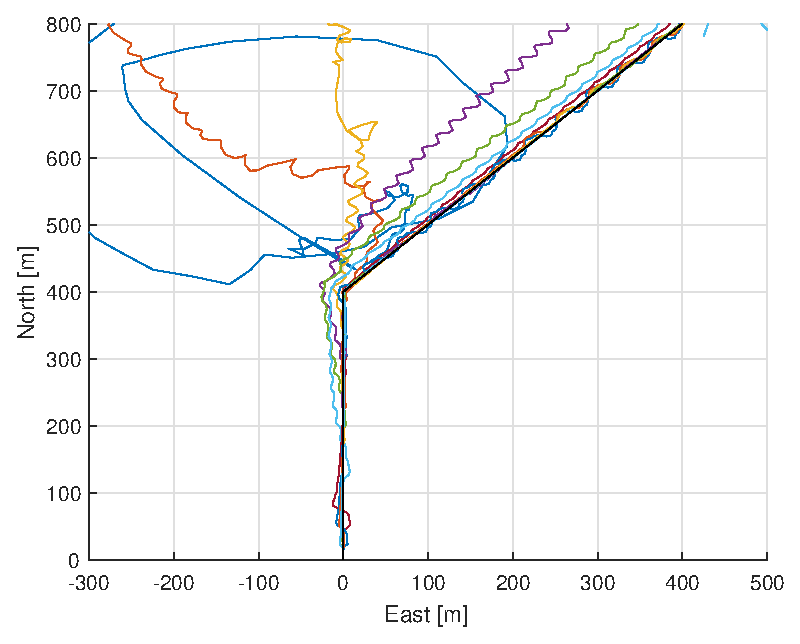
\includegraphics[width=0.8\textwidth, keepaspectratio=true]{../../results/opt/horizon/lin_45deg/fig/camera_position.eps}}}
	\qquad
	\makebox[\textwidth][c]{
	\subfloat[Subfigure 2][Curved $45\degree$ turn with $200$m radius.]{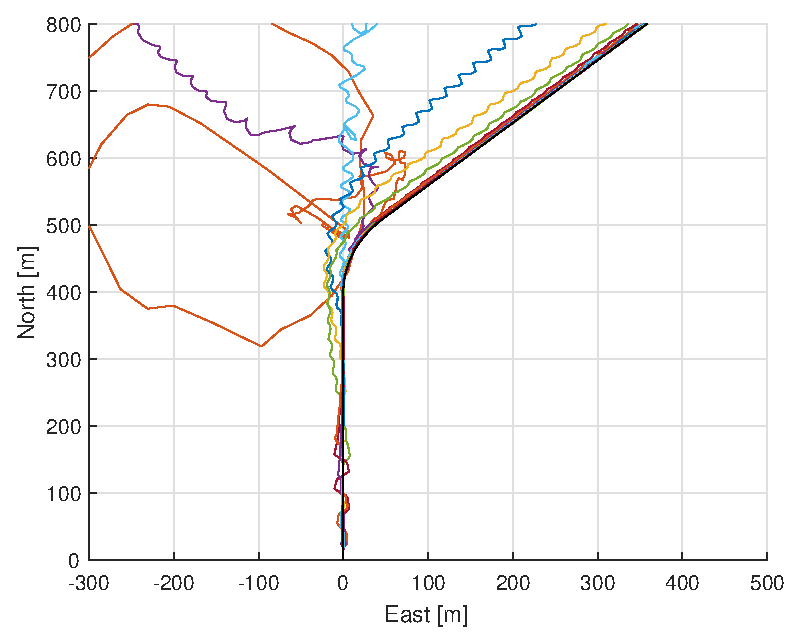
\includegraphics[width=0.8\textwidth, keepaspectratio=true]{../../results/opt/horizon/cur_45deg_200m/fig/camera_position.eps}}}
	\caption{The camera position during the two turns with horizon lengths varying from 10 to 140.}
	\label{fig:horizon_camera_position}
\end{figure}


%% Duration
\begin{figure}
	\makebox[\textwidth][c]{
	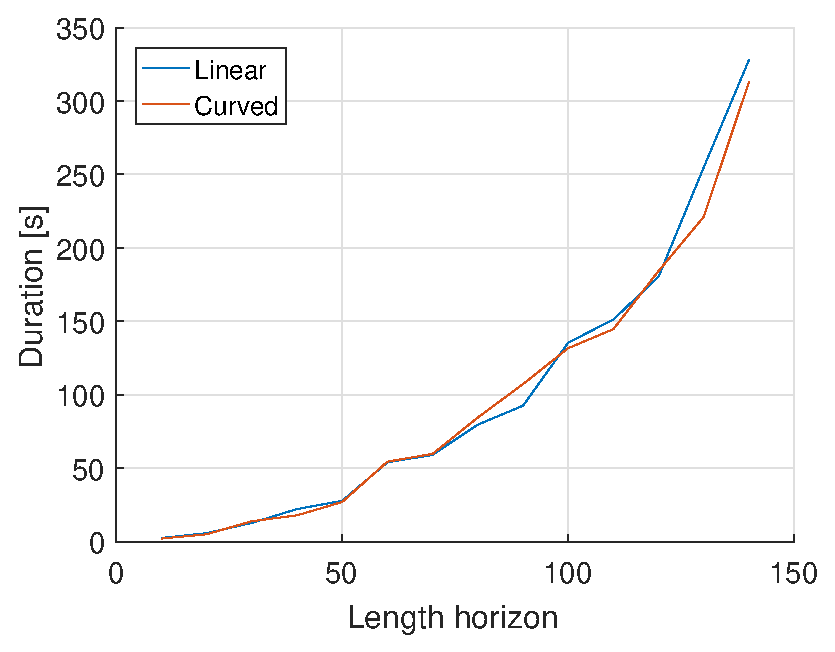
\includegraphics[width=0.8\textwidth, keepaspectratio=true]{../../results/opt/horizon/duration_both.eps}}
	\caption{Duration of each optimization with different horizon length.}
	\label{fig:horizon_duration}
\end{figure}